\documentclass{article}[18pt]
\ProvidesPackage{format}
%Page setup
\usepackage[utf8]{inputenc}
\usepackage[margin=0.7in]{geometry}
\usepackage{parselines} 
\usepackage[english]{babel}
\usepackage{fancyhdr}
\usepackage{titlesec}
\hyphenpenalty=10000

\pagestyle{fancy}
\fancyhf{}
\rhead{Sam Robbins}
\rfoot{Page \thepage}

%Characters
\usepackage{amsmath}
\usepackage{amssymb}
\usepackage{gensymb}
\newcommand{\R}{\mathbb{R}}

%Diagrams
\usepackage{pgfplots}
\usepackage{graphicx}
\usepackage{tabularx}
\usepackage{relsize}
\pgfplotsset{width=10cm,compat=1.9}
\usepackage{float}

%Length Setting
\titlespacing\section{0pt}{14pt plus 4pt minus 2pt}{0pt plus 2pt minus 2pt}
\newlength\tindent
\setlength{\tindent}{\parindent}
\setlength{\parindent}{0pt}
\renewcommand{\indent}{\hspace*{\tindent}}

%Programming Font
\usepackage{courier}
\usepackage{listings}
\usepackage{pxfonts}

%Lists
\usepackage{enumerate}
\usepackage{enumitem}

% Networks Macro
\usepackage{tikz}


% Commands for files converted using pandoc
\providecommand{\tightlist}{%
	\setlength{\itemsep}{0pt}\setlength{\parskip}{0pt}}
\usepackage{hyperref}

% Get nice commands for floor and ceil
\usepackage{mathtools}
\DeclarePairedDelimiter{\ceil}{\lceil}{\rceil}
\DeclarePairedDelimiter{\floor}{\lfloor}{\rfloor}

% Allow itemize to go up to 20 levels deep (just change the number if you need more you madman)
\usepackage{enumitem}
\setlistdepth{20}
\renewlist{itemize}{itemize}{20}

% initially, use dots for all levels
\setlist[itemize]{label=$\cdot$}

% customize the first 3 levels
\setlist[itemize,1]{label=\textbullet}
\setlist[itemize,2]{label=--}
\setlist[itemize,3]{label=*}

% Definition and Important Stuff
% Important stuff
\usepackage[framemethod=TikZ]{mdframed}

\newcounter{theo}[section]\setcounter{theo}{0}
\renewcommand{\thetheo}{\arabic{section}.\arabic{theo}}
\newenvironment{important}[1][]{%
	\refstepcounter{theo}%
	\ifstrempty{#1}%
	{\mdfsetup{%
			frametitle={%
				\tikz[baseline=(current bounding box.east),outer sep=0pt]
				\node[anchor=east,rectangle,fill=red!50]
				{\strut Important};}}
	}%
	{\mdfsetup{%
			frametitle={%
				\tikz[baseline=(current bounding box.east),outer sep=0pt]
				\node[anchor=east,rectangle,fill=red!50]
				{\strut Important:~#1};}}%
	}%
	\mdfsetup{innertopmargin=10pt,linecolor=red!50,%
		linewidth=2pt,topline=true,%
		frametitleaboveskip=\dimexpr-\ht\strutbox\relax
	}
	\begin{mdframed}[]\relax%
		\centering
		}{\end{mdframed}}



\newcounter{lem}[section]\setcounter{lem}{0}
\renewcommand{\thelem}{\arabic{section}.\arabic{lem}}
\newenvironment{defin}[1][]{%
	\refstepcounter{lem}%
	\ifstrempty{#1}%
	{\mdfsetup{%
			frametitle={%
				\tikz[baseline=(current bounding box.east),outer sep=0pt]
				\node[anchor=east,rectangle,fill=blue!20]
				{\strut Definition};}}
	}%
	{\mdfsetup{%
			frametitle={%
				\tikz[baseline=(current bounding box.east),outer sep=0pt]
				\node[anchor=east,rectangle,fill=blue!20]
				{\strut Definition:~#1};}}%
	}%
	\mdfsetup{innertopmargin=10pt,linecolor=blue!20,%
		linewidth=2pt,topline=true,%
		frametitleaboveskip=\dimexpr-\ht\strutbox\relax
	}
	\begin{mdframed}[]\relax%
		\centering
		}{\end{mdframed}}
\lhead{Software Engineering}


\begin{document}
\begin{center}
\underline{\huge Process Improvement}
\end{center}
\section{Approaches to improvement}
The process maturity approach:
\begin{itemize}
	\item Focuses on improving processes and project management and introducing good software engineering practice
	\item The level of process maturity reflects the extent to which good technical and management practice has been adopted in organizational software development processes
\end{itemize}
The agile approach:
\begin{itemize}
	\item Focuses on iterative development and the reduction of overheads in the software process
	\item The primary characteristics of agile methods are rapid delivery of functionality and responsiveness to changing customer requirements
\end{itemize}
\section{Factors affecting software product quality}
\begin{itemize}
	\item People quality
	\item Process quality
	\item Cost, time and schedule
	\item Developmental technology
\end{itemize}
\section{Process improvement stages}
Process measurement:
\begin{itemize}
	\item Attributes of the current process are measured. These are a baseline for assessing improvements. Wherever possible, quantitative process data should be collected
\end{itemize}
Process analysis:
\begin{itemize}
	\item The current process is assessed and bottlenecks and weaknesses are identified
\end{itemize}
Process change:
\begin{itemize}
	\item Changes to the process that have been identified during the analysis are introduced
\end{itemize}
\section{Process measurement}
This is done by the Goal Question Metric (GQM) paradigm
\begin{enumerate}
	\item Why are we introducing process improvement
	\item What info do we collect to help ID and assess improvement
	\item What process and product measures will provide this information
\end{enumerate}
\begin{center}
	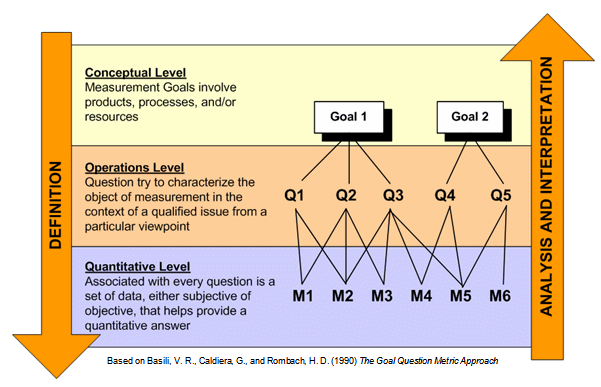
\includegraphics[scale=0.7]{GQM}
\end{center}
\section{Process change}
Involves making modifications to existing processes\\
This may involve:
\begin{itemize}
	\item Introducing new practices, methods or processes
	\item Changing the ordering of process activities
	\item Introducing or removing deliverables
	\item Introducing new roles or responsibilities
\end{itemize}
Change should be driven by measurable goals
\section{Process capability assessment}
Intended as a means to assess the extent to which an organisation's processes follow best practice\\
\\
Processes are assigned a capability assessment level of 1-5 with 5 being the highest:
\begin{itemize}
	\item Each level has an associated set of process areas and generic goals
	\item Lower levels achieved by using good practice whilst higher levels require a commitment to process measurement and improvement
\end{itemize}
By providing a means for assessment, it is possible to identify areas of weakness for process improvement\\
\\
There have been various process assessment and improvement models but the SEI work has been the most influential
\section{CMMI}
\begin{definition}[CMMI]
	Capability Maturity Model Integration, a framework made by the SEI for assessing the capabilities of software contractors
\end{definition}
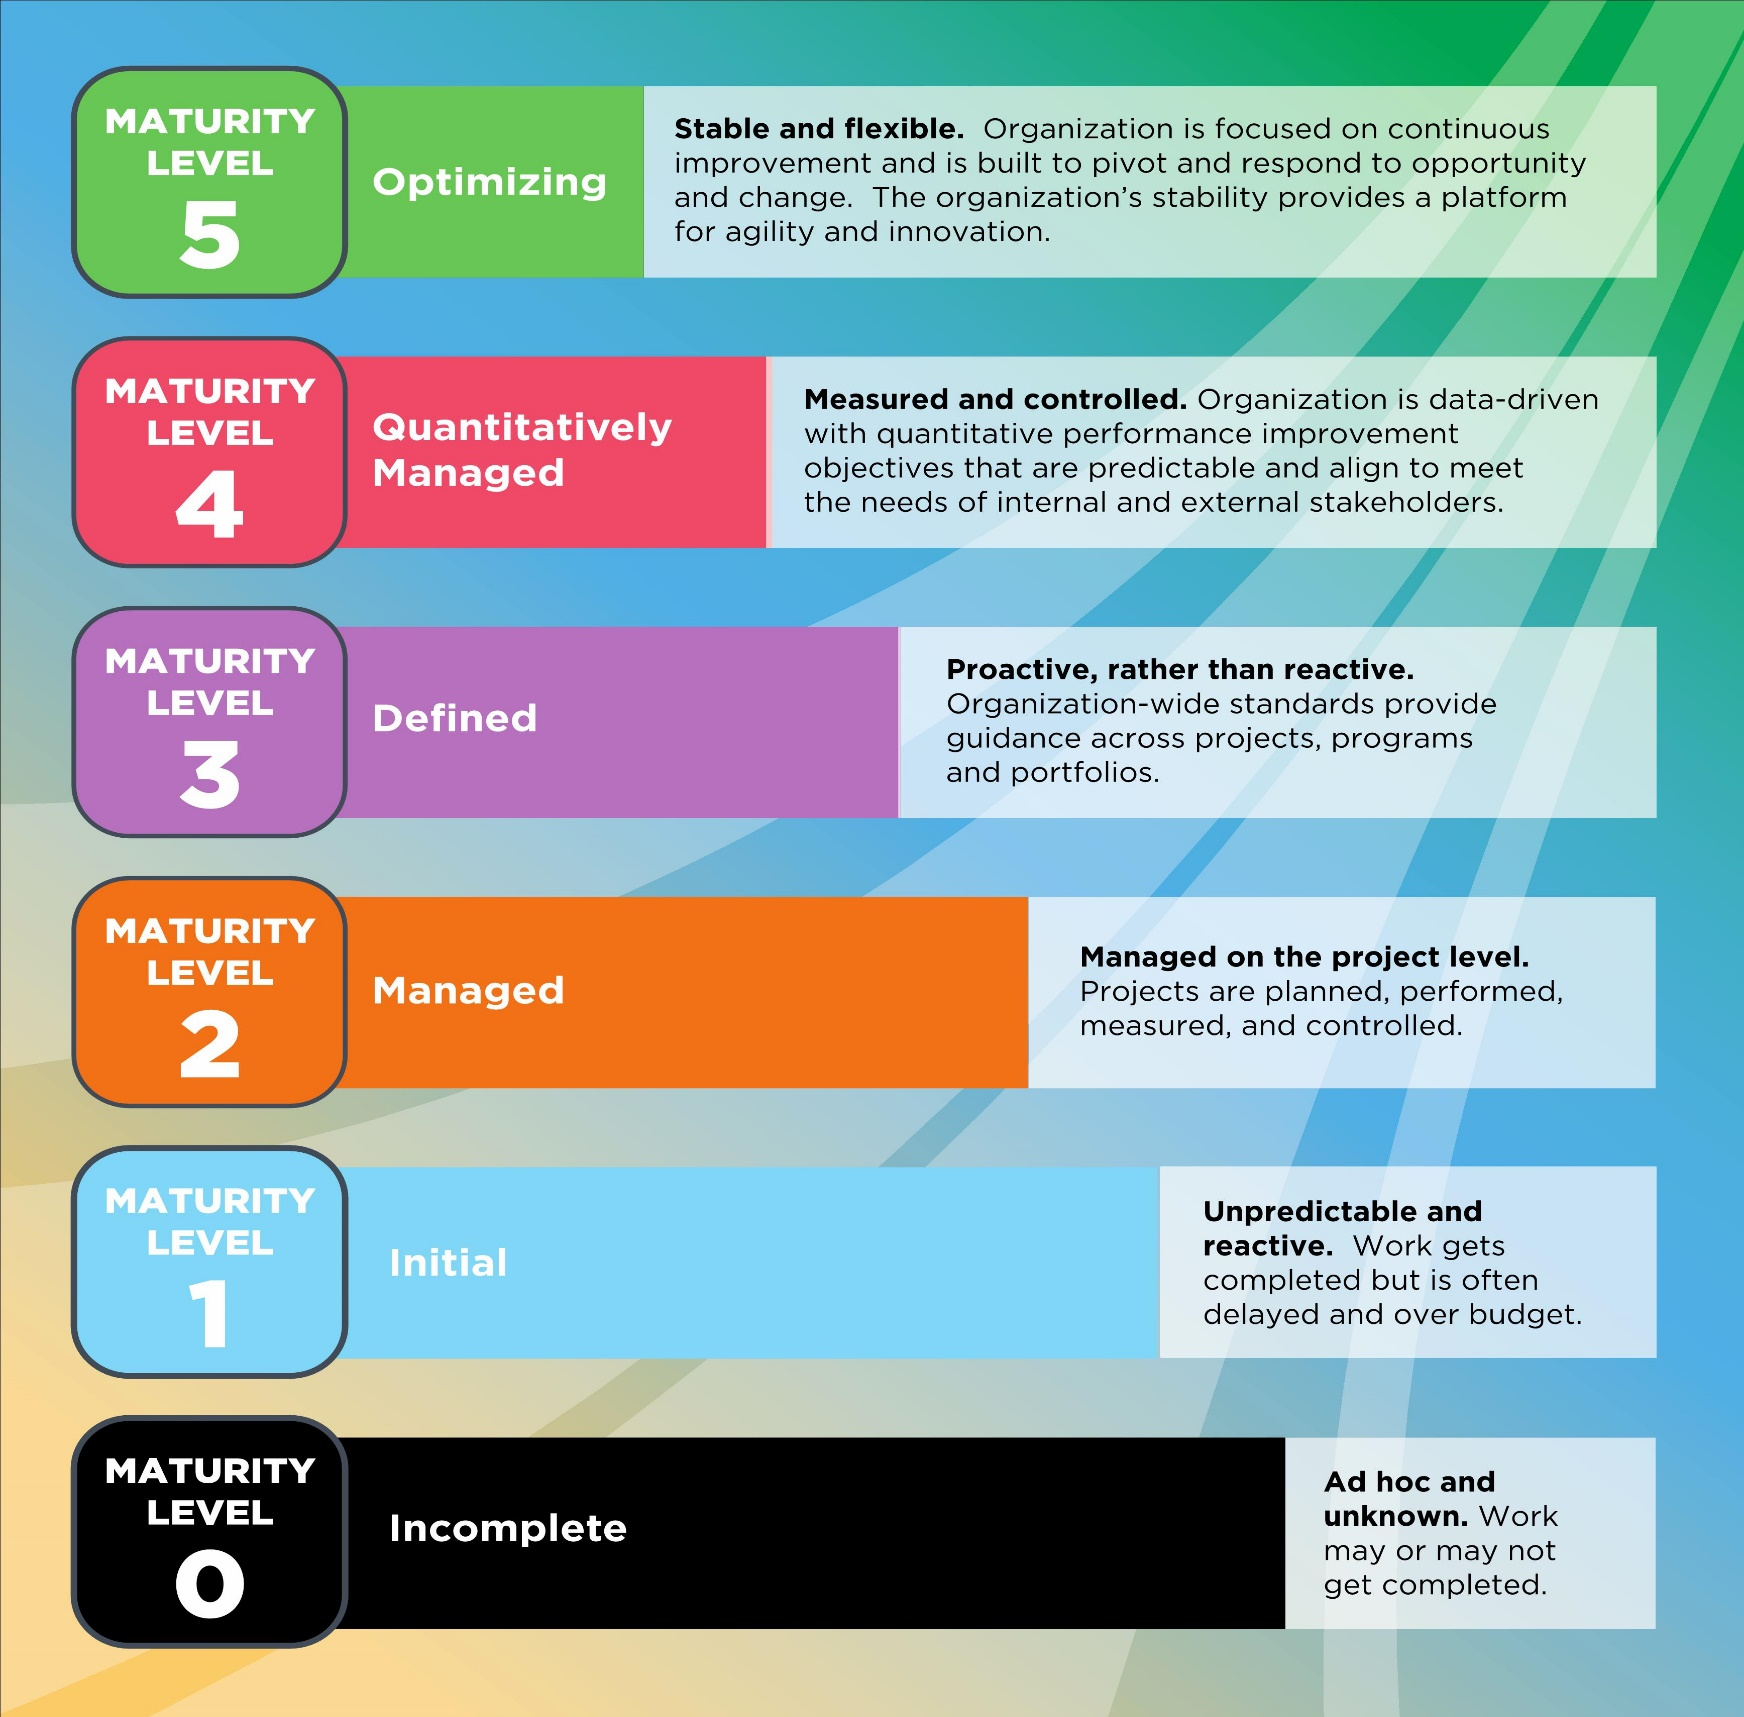
\includegraphics[scale=0.5]{CMMI}
\subsection{Level 1 - Initial}
Describes a software development process that is ad hoc or even chaotic\\
\\
It is difficult even to write down or depict the overall process\\
\\
No key process areas at this level\\
\\
Example questions to be at level 1:
\begin{itemize}
	\item Is a mechanism used for controlling changes to the software requirements
	\item Does the software quality assurance function have a management reporting channel separate from the software development project management
	\item Is there a software configuration control function for each project that involves software development
	\item Is a formal process used in the management review of each software development prior to making contractual commitments
	\item Is a formal procedure used to make estimates of software size
\end{itemize}
\subsection{Level 2 - Managed}
Identifying the inputs and outputs of the process, the constraints and the resources used to produce final product\\
\\
Requirements are managed and processes are planned, performed, monitored and controlled for individual projects\\
\\
Is a level of discipline to stick to these processes
\subsection{Level 3 - Defined}
Management and engineering activities are documented, standardized and integrated into each other
\subsection{Level 4 - Quantitatively managed}
\begin{definition}[Quantitatively managed]
	Process directs its effort at product quality
\end{definition}
Processes are measured by collecting detailed data on the process and their quality. Statistical and other quantitative techniques used and therefore quantitatively predictable.\\
\\
These measures are used to support fact based decision making in the future\\
\\
Quality and process performance is understood in statistical terms and is managed throughout the life of the process
\subsection{Level 5 - Optimised}
Quantitative feedback is incorporated in the process to produce continuous process improvement.\\
\\
Focused on continually improving process performance through both incremental and innovative technological improvements
\section{Immature vs Mature organisation}
Characteristics of an immature organisation:
\begin{itemize}
	\item Process improvised during project
	\item Approved processes being ignored
	\item Reactive, not proactive
	\item Unrealistic budget and schedule
	\item Quality sacrificed for schedule
	\item No objective measure of quality
\end{itemize}
Characteristics of a mature organisation:
\begin{itemize}
	\item Inter group communication and coordination
	\item Work accomplished according to plan
	\item Practices consistent with processes
	\item Processes updated as necessary
	\item Well defined roles/responsibilities
	\item Management formally commits
\end{itemize}
\section{MMMs}
Management Maturity Model - CMMI is the de facto standard in software engineering\\
\\
Others:
\begin{itemize}
	\item ITSM/ITIL
	\item Agile
	\item DevOps
	\item MDM (Master Data Model)
\end{itemize}


\end{document}